\section{Parsiranje gramatika programskih jezika}
\label{sec:ParsingGrammars}

Pretpostavljajući da imamo gramatiku proizvoljnog programskog jezika, postavlja se pitanje: \emph{Da li je moguće definisati postupak i zatim napraviti program koji će generisati kodove leksera i parsera napisane u određenom programskom jeziku za proizvoljnu gramatiku datu na ulazu?}. Odgovor je potvrdan i postoji veliki broj alata koji se mogu koristiti u ove svrhe, od kojih je navedeno par njih u odeljcima ispod.


\subsection{GNU Bison}
\label{subsec:GNUBison}

\emph{GNU Bison} \cite{GNUBison} je generator parsera i deo GNU projekta \cite{GNUProject}, često referisan samo kao \emph{Bison}. Bison generiše parser na osnovu korisnički definisanih kontekstno slobodnih gramatika \cite{ContextFreeGrammars}, upozoravajući pritom na dvosmislenosti prilikom parsiranja ili nemogućnost primena gramatičkih pravila. Generisani parser je najčešće C a ređe C++ kod, mada se u vreme pisanja ovog rada eksperimentiše sa Java podrškom. Generisani kodovi su u potpunosti prenosivi i ne zahtevaju specifične kompajlere. Bison može da, osim podrazumevanih \emph{LALR(1)} \cite{LALR1} parsera, generiše i kanoničke \emph{LR} \cite{LR}, \emph{IELR(1)} \cite{IELR1} i \emph{GLR} \cite{GLR} parsere.

\subsection{Flex}
\label{subsec:Flex}

\emph{Flex} \cite{Flex} je kreiran kao alternativa \emph{lex}-u \cite{LexYacc}, Flex generiše samo leksere pa se stoga najčešće koristi u kombinaciji sa drugim alatima koji mogu da generišu parsere, kao što je \emph{BYACC}, opisan u nastavku.

\subsection{BYACC}
\label{subsec:BYACC}

\emph{Berkeley YACC}, skraćeno \emph{BYACC} \cite{BYACC}, pisan po ANSI C standardu i otvorenog koda, se smatra od strane mnogih kao \textit{najbolja varijanta YACC-a} \cite{LexYacc}. BYACC dozvoljava tzv. \emph{reentrant} kod - memorija je deljenja između poziva pa je bezbedno konkurentno izvršavanje koda - na način kompatibilan sa Bison-om i to je delom razlog njegove popularnosti.

\subsection{ANTLR}
\label{subsec:ANTLR}
\emph{Another Tool for Language Recognition}, ili kraće \emph{ANTLR} \cite{ANTLR}, je generator \emph{LL(*)} \cite{LLStar} leksera i parsera pisan u programskom jeziku Java sa intuitivnim interfejsom za obilazak stabla parsiranja. Verzija $3$ podržava generisanje parsera u jezicima Ada95, ActionScript, C, C\#, Java, JavaScript, Objective-C, Perl, Python, Ruby, i Standard ML, dok verzija $4$ u vreme pisanja ovog rada samo generiše parsere u narednim jezicima: Java, C\#, C++, JavaScript, Python, Swift i Go.

ANTLR verzije $4$ je izabran u ovom radu zbog svoje jednostavnosti, intuitivnosti i podrške za mnoge moderne programske jezike. Verzija $4$ je izabrana umesto verzije $3$ po preporuci autora, na osnovu eksperimentalne analize brzine i pouzdanosti verzije $4$ u odnosu na verziju $3$. Lekseri i parseri za ulazne gramatike će u implementaciji biti generisani u programskom jeziku C\#.

Parseri generisani koristeći ANTLR koriste novu tehnologiju koja se naziva \emph{Prilagodljiv LL(*)} (engl. \emph{Adaptive LL(*)}) ili \emph{ALL(*)} \cite{ANTLRReference}, dizajniranu od strane Terensa Para, autora ANTLR-a, i Sema Harvela. \emph{ALL(*)} vrši \emph{dinamičku analizu} gramatike u fazi izvršavanja, dok su starije verzije radile analizu pre pokretanja parsera, tzv. \emph{statičku analizu}. Ovaj pristup je takođe efikasniji zbog značajno manjeg prostora ulaznih sekvenci.

Najbolji aspekt ANTLR-a je lakoća definisanja gramatičkih pravila koji opisuju sintaksne konstrukte nalik na aritmetičkim izrazima u programskim jezicima. Primer jednostavnog pravila za definisanje aritmetičkog izraza je dat na slici \ref{fig:ANTLRExpressions}. Pravilo \texttt{exp} je levo rekurzivno jer barem jedna od njegovih alternativnih definicija referiše na baš pravilo \texttt{exp}. ANTLR4 automatski zamenjuje levo rekurzivna pravila u nerekurzivne ekvivalente. Jedini zahtev koji mora biti ispunjen je da levo rekurzivna pravila moraju biti \emph{direktna} - da pravila odmah referišu sama sebe. Pravila ne smeju referisati drugo pravilo sa leve strane definicije takvo da se eventualno kroz rekurziju stigne nazad do pravila od kog se krenulo bez poklapanja sa nekim tokenom.

\begin{figure}[h!]
    \begin{lstlisting}[language={}]
    exp : (exp)
        | exp '*' exp
        | exp '+' exp
        | INT
        ;
    \end{lstlisting}
    \caption{Definicija uprošćenog aritmetičkog izraza u ANTLR4 gramatici.}
    \label{fig:ANTLRExpressions}
\end{figure}


\subsubsection{Preduslovi za pokretanje ANTLR4}
\label{subsubsec:ANTLRInstallation}

Kako bi ANTLR generisao parser u proizvoljnom programskom jeziku, potrebno je instalirati ANTLR i imati \emph{Java Runtime Environment} (skr. \emph{JRE}) instaliran na sistemu i dostupan globalno pokretanjem putem komande \texttt{java}. Instalacija se sastoji od preuzimanja najnovijeg \emph{.jar} fajla
\footnote{Takođe je moguće kompajlirati izvorni kod dostupan na servisu GitHub \url{https://github.com/antlr/antlr4}}, sa zvanične stranice \cite{ANTLR} ili recimo korišćenjem \emph{curl} alata: 
\begin{lstlisting}[language={}]
$ curl -O http://www.antlr.org/download/antlr-4-complete.jar
\end{lstlisting}

Na UNIX sistemima moguće je kreirati alias \texttt{antlr4} ili \emph{shell} skript unutar direktorijuma \texttt{/usr/local/bin} sa imenom \texttt{antlr4} koji će pokrenuti \emph{.jar} fajl na sledeći način (pretpostavljajući da se \emph{.jar} fajl nalazi u direktorijumu \texttt{/usr/local/lib}):
\begin{lstlisting}[language={}]
#!/bin/sh
java -cp "/usr/local/lib/antlr4-complete.jar:$CLASSPATH" org.antlr.v4.Tool $*
\end{lstlisting}

Na Windows sistemima moguće je kreirati \emph{batch} skript sa imenom \texttt{antlr4.bat} koji će pokrenuti ANTLR4, na sledeći način (pretpostavljajući da se \emph{.jar} fajl nalazi u direktorijumu \texttt{C:\textbackslash{}lib}):
\begin{lstlisting}[language={}]
java -cp C:\lib\antlr-4-complete.jar;%CLASSPATH% org.antlr.v4.Tool %*
\end{lstlisting}

Ukoliko su aliasi ili skript fajlovi imenovani kao iznad, moguće je iz komandne linije pojednostavljeno pokretati ANTLR4:  
\begin{lstlisting}[language={}]
$ antlr4
ANTLR Parser Generator Version 4.0
-o ___    specify output directory where all output is generated
-lib ___  specify location of .tokens files
...
\end{lstlisting}

Dodatno, za Unix sisteme \footnote{Za Windows operativni sistem je moguće kreirati \emph{batch} skript po opisu na \url{https://github.com/antlr/antlr4/blob/master/doc/getting-started.md}.}, moguće je kreirati dodatni alias \texttt{grun} (ili alternativno, kreirati \texttt{shell script}) za biblioteku \texttt{TestRig}. Biblioteka TestRig se može koristiti za brzo testiranje parsera - moguće je pokrenuti parser od bilo kog pravila i dobiti izlaz parsera u raznim formatima. TestRig dolazi uz ANTLR \texttt{.jar} fajl i moguće je napraviti prečicu za brzo pokretanje (nalik na ANTLR alias):
\begin{lstlisting}[language={}]
$ alias grun='java -cp "/usr/local/lib/antlr-4-complete.jar:$CLASSPATH" org.antlr.v4.gui.TestRig'
\end{lstlisting}


\subsection{Generisanje parsera koristeći ANTLR4}
\label{subsec:ANTLRParserGeneration}

Prvi korak u izradi aplikacije koja u sebi koristi parsiranje nekog jezika je definisanje gramatike jezika i kreiranje leksera i parsera za isti. U nastavku će biti opisan proces kreiranja interfejsa za parsiranje programa pisanih u pseudo-programskom jeziku (u nastavku \emph{pseudo-jezik}), nalik na pseudokod. Ovako dobijeni interfejs će moći da se koristi u opšte svrhe, za potrebe ovog rada će se koristiti za generisanje AST stabla za program pisan u pseudo-jeziku.

Definišimo gramatiku pseudo-jezika prateći ANTLR pravila za definisanje gramatika. Kao i za svaki drugi programski jezik, treba obezbediti da postoje određeni koncepti koji se pojavljuju u programskim jezicima: \emph{identifikatori}, \emph{izrazi}, \emph{naredbe}, \emph{funkcije} i slično. Za sada se fokusirajmo na naredbe, kao samostalne izvršive jedinice koda. Stoga program možemo smatrati kao niz naredbi. U nekim slučajevima će biti potrebno definisanje kompleksnih naredbi koje se sastoje od više drugih naredbi, i ovakve složene naredbe ćemo zvati \emph{blok} ili \emph{blok naredbi}. Stoga, radi konzistentnosti, program će biti blok naredbi. Kako bismo označili da su naredbe deo bloka naredbi, koristićemo reči \texttt{begin} i \texttt{end}, osim ukoliko je reč o samo jednoj naredbi. Ovakve situacije rešavamo definisanjem \emph{alternativa} u definiciji pravila - više definicija razdvojenih simbolom \texttt{|}. Specijalne reči kao što su \texttt{begin} i \texttt{end} će biti rezervisane reči našeg pseudo-jezika, tzv. \emph{ključne reči}. Na slici \ref{fig:PseudoDef1} se može videti definicija programa \footnote{Drugim rečima, jedan program u pseudo-jeziku je jedinica prevođenja, pa je zato pravilo nazvano \emph{unit}.} i bloka naredbi pseudo-jezika, pri čemu se ključne reči u pravilima navode između apostrofa. ANTLR dozvoljava jednostavne definicije pravila u kojima figuriše promenljiv broj drugih pravila, pri čemu se koriste simboli kao u regularnim izrazima \footnote{U regularnim izrazima, simbol \texttt{a?} označava opciono pojavljivanje simbola \texttt{a}, simbol \texttt{a+} označava jedno ili više pojavljivanja simbola \texttt{a}, a simbol \texttt{a*} označava proizvoljan broj pojavljivanja simbola \texttt{a} - kombinacija simbola \texttt{?} i \texttt{+}.}, što je iskorišćeno za definiciju pravila bloka naredbi. \texttt{NAME} predstavlja ime programa, što je zapravo identifikator. Identifikatore ćemo definisati kasnije, za sada možemo posmatrati identifikator kao nisku karaktera s tim što će postojati restrikcije vezane za to koji karakteri se mogu naći unutar identifikatora ali o tome će biti reči kasnije.

\begin{figure}[h!]
    \begin{lstlisting}[language={}]
    unit
        : 'algorithm' NAME block EOF
        ;
    
    block
        : 'begin' statement+ 'end'
        | statement
        ;
    \end{lstlisting}
    \caption{Definicija jedinice prevođenja i bloka naredbi za pseudo-jezik.}
    \label{fig:PseudoDef1}
\end{figure}

Sledeći korak je definisanje naredbe pseudo-jezika. Slično kao i u drugim programskim jezicima, potrebno je podržati koncept deklaracije promenljive, dodele vrednosti izraza promenljivoj, naredbe kontrole toka - grananje i petlje. Na slici \ref{fig:PseudoDef2} je definisano šta se sve smatra jednom naredbom. Naredbe mogu biti i prazne, što je označeno ključnom rečju \texttt{pass}. Iz definicije naredbe sa slike se jasno vidi šta sve može biti naredba (prateći redosled alternativa pravila):
\begin{itemize}
    \item deklaracija
    \item dodela
    \item poziv funkcije (označen kao \texttt{cexp}, skraćeno od \emph{function call expression}) \footnote{Funkcije mogu vratiti vrednosti pa se stoga njihovi pozivi mogu naći u izrazima - dakle poziv funkcije je validan izraz (stoga \texttt{expression} u imenu \texttt{function call expression}). Naravno, ta vrednost se može ignorisati ili pak sama funkcija može biti takva da nema povratnu vrednost već je samo neophodno izvršiti je zbog sporednih efekata.}
    \item vraćanje vrednosti izraza (ključna vrednost \texttt{return}) iz funkcije
    \item prekidanje izvršavanja davanjem poruke o grešci
    \item naredba grananja
    \item \emph{while} petlja
    \item \emph{repeat-until} petlja
    \item inkrementiranje/dekrementiranje vrednosti promenljive
\end{itemize}
    
\begin{figure}[h!]
    \begin{lstlisting}[language={}]
    statement
        : 'pass'
        | declaration
        | assignment
        | cexp
        | 'return' exp
        | 'error' STRING
        | 'if' exp 'then' block ('else' block)? 
        | 'while' exp 'do' block 
        | 'repeat' block 'until' exp
        | ('increment' | 'decrement') var	
        ;
    \end{lstlisting}
    \caption{Definicija naredbe za pseudo-jezik.}
    \label{fig:PseudoDef2}
\end{figure}

Deklaracija, prikazana na slici \ref{fig:PseudoDef3}, uvodi pojavljivanje simbola datog preko identifikatora \texttt{NAME} kao oznaku za promenljivu, funkciju ili proceduru - funkciju bez povratne vrednosti. Svaka promenljiva mora biti određenog tipa, što se postiže pravilom \texttt{type}. Promenljivoj se, opciono, može pridružiti početna vrednost, drugim rečima promenljiva se može \emph{inicijalizovati} tako da joj se pridruži vrednost nekog izraza. Procedure i funkcije imaju opcione parametre, vrednosti izraza koje im se prosleđuju kasnije u pozivu kao argumenti. Lista parametara, takođe prikazana na slici \ref{fig:PseudoDef3}, se navodi kao lista proizvoljno mnogo parova \texttt{NAME : type}, što se vidi iz definicije pravila \texttt{parlist}.

\begin{figure}[h!]
    \begin{lstlisting}[language={}]
    declaration
        : 'declare' type NAME ('=' exp)? 
        | 'procedure' NAME '(' parlist? ')' block 
        | 'function' NAME '(' parlist? ')' 'returning' type block 
        ;

    parlist
        : NAME ':' type (',' NAME ':' type)*
        ;
    \end{lstlisting}
    \caption{Definicija deklaracije za pseudo-jezik.}
    \label{fig:PseudoDef3}
\end{figure}

Identifikatori su niske karaktera koje predstavljaju ime koje odgovara određenoj memorijskoj adresi. Identifikatori se koriste umesto sirovih vrednosti adresa kako bi kod bio čitljiviji i lakši za pisanje - na nivou asemblera se većinom koriste adrese ili automatski generisane oznake. Na slici \ref{fig:PseudoDef4} se može videti definicija identifikatora. Identifikator se sastoji od slova, cifara i simbola \texttt{\_}, s tim što ne sme početi cifrom. Ovo je konvencija koju prati dosta jezika, uključujući programski jezik C. Primetimo da je identifikator nešto što bi lekser trebalo da prepozna tokom tokenizacije. Međutim, kada definišemo gramatiku od koje će ANTLR praviti lekser i parser, možemo i tokene definisati preko gramatičih pravila dajući regularni izraz za njihovo poklapanje. Listovi stabla parsiranja su uvek tokeni, drugim rečima se nazivaju i \emph{terminalni simboli}. Tokeni se, naravno, mogu naći bilo gde u stablu parsiranja.

\begin{figure}[h!]
    \begin{lstlisting}[language={}]
    NAME
        : [a-zA-Z_][a-zA-Z_0-9]*
        ;
    \end{lstlisting}
    \caption{Definicija identifikatora za pseudo-jezik.}
    \label{fig:PseudoDef4}
\end{figure}

Pošto želimo da pseudo-jezik bude strogo tipiziran, potreban je koncept tipa (što smo videli u deklaracijama), čija je definicija data na slici \ref{fig:PseudoDef5}. Tip može biti \emph{primitivan} (drugim rečima \emph{prost}) ili \emph{složen}. Primitivni tipovi su podržani u samoj sintaksi jezika - u našem slučaju brojevi i niske. Brojevi mogu biti celi ili realni. U složene tipove spadaju korisnički definisani tipovi (sa imenom \texttt{NAME}, u četvrtoj alternativi pravila \texttt{typename} sa slike \ref{fig:PseudoDef5}) i kolekcije. Od kolekcija su podržani nizovi, liste i skupovi. Prilikom definicije kolekcije mora se navesti tip elemenata kolekcije i taj tip mora biti uniforman - isti za sve elemente kolekcije. 

\begin{figure}[h!]
    \begin{lstlisting}[language={}]
    type 
        : typename 'array'?
        | typename 'list'?
        | typename 'set'?
        ;

    typename 
        : 'integer' 
        | 'real' 
        | 'string' 
        | NAME 
        ;
    \end{lstlisting}
    \caption{Definicija tipa podataka za pseudo-jezik.}
    \label{fig:PseudoDef5}
\end{figure}

Izrazi, iako se definišu rekurzivno, se mogu posmatrati kao kombinacija promenljivih, operatora i poziva funkcija sa odlikom da se mogu \emph{evaluirati}, tj. moguće je izračunati njegovu vrednost. Iz definicije pravila \texttt{exp} na slici \ref{fig:PseudoDef6}, mogu se uočiti tipovi izraza, pri čemu nije vođeno računa o matematičkom prioritetu operatora, radi jednostavnosti. Izraz može biti \emph{literal}, koji predstavlja konstantu, bilo brojevnu, logičku ili nisku karaktera. Promenljive, definisane pravilom \texttt{var} su takođe izrazi, jer se trenutna vrednost promenljive posmatra kao vrednosti izraza. Primetimo da promenljiva može biti kolekcijskog tipa, u kom slučaju se navodi redni broj elementa nakon identifikatora promenljive - taj redni broj može biti rezultat evaluacije drugog izraza, ali ne bilo kakvog, stoga se u pravilu \texttt{iexp} definiše šta sve može biti korišćeno da se indeksira element kolekcije. Izrazima se može dati prioritet pomoću zagrada, što se vidi u trećoj alternativi pravila \texttt{exp}. U naredne tri alternative su opisani tipovi izraza: aritmetički, relacioni i logički. Aritmetički izrazi su vezani aritmetičkim operatorima definisanim preko pravila \texttt{aop}, slično važi i za ostala dva tipa. Svi tipovi izraza navedeni iznad su binarni, što znači da operatori zahtevaju dva argumenta. Postoje i unarni izrazi, od kojih su podržane promena znaka i logička negacija, što se vidi iz pravila \texttt{uop}.

\begin{figure}[h!]
    \begin{lstlisting}[language={}]
    exp
        : literal 
        | var
        | '(' exp ')'
        | exp aop exp
        | exp rop exp
        | exp lop exp
        | uop exp
        | cexp
        ;

    var 
        : NAME ('[' iexp ']')?
        ;
    
    iexp 
        : literal
        | var
        | aexp
        ;

    cexp
        : 'call' NAME '(' explist? ')'
        ;

    explist
        : exp (',' exp)*
        ;

    aop : '+' | '-' | '*' | '/' | 'div' | 'mod' ;
    rop : '>' | '>=' | '<' | '<=' | '==' | '=/=' ;
    lop : 'and' | 'or' ;
    uop : '-' | 'not' ;
    \end{lstlisting}
    \caption{Definicija izraza za pseudo-jezik.}
    \label{fig:PseudoDef6}
\end{figure}

Definicija literala je prikazana na slici \ref{fig:PseudoDef7}. Literali mogu bili istinitosne konstante \texttt{True} i \texttt{False}, brojevne konstante ili niske karaktera. Brojevne konstante mogu bili celobrojni ili realni dekadni brojevi. Realne konstatne je moguće definisati u fiksnom ili pokretnom zarezu. Niske se mogu definisati između navodnika ili apostrofa. Pritom, kao i u modernim programskim jezicima, moguće je navesti sekvence koje predstavljaju specijalne karaktere kao što su novi red, tabulator itd. Oznaka \texttt{fragment} označava optimizaciju, naime nije potrebno da postoji na primer pravilo \texttt{Digit}, već samo dajemo simbol za regularni izraz koji će se koristiti u više drugih pravila i poklapati jednu dekadnu cifru.

\begin{figure}[h!]
    \begin{lstlisting}[language={}]
    literal : 'True' | 'False' | INT | FLOAT | STRING ;

    STRING
        : '"' ( EscapeSequence | ~('\\'|'"') )* '"' 
        ;

    fragment
    EscapeSequence
        : '\\' [abfnrtvz"'\\]
        | '\\' '\r'? '\n'
        ;

    INT
        : Digit+
        ;

    FLOAT
        : Digit+ '.' Digit* ExponentPart?
        | '.' Digit+ ExponentPart?
        | Digit+ ExponentPart
        ;

    fragment
    ExponentPart
        : [eE] [+-]? Digit+
        ;

    fragment
    Digit
        : [0-9]
        ;
    \end{lstlisting}
    \caption{Definicija konstanti za pseudo-jezik.}
    \label{fig:PseudoDef7}
\end{figure}

Poslednje što treba definisati je sve ono što lekser treba da preskoči tokom prolaska kroz izvorni kod programa. To su beline (nevidljivi karakteri kao što su razmaci, tabulatori i novi redovi) i komentari. Definicije ovih pravila se mogu videti na slici \ref{fig:PseudoDef8}. Vidimo da se u njima koristi posebna oznaka \texttt{-> skip}, koja predstavlja instrukcije lekseru da preskoči sve ono što ovo pravilo poklopi. Komentari su u stilu kao u programskom jeziku C (ali naravno, isti stil se koristi i u mnogim jezicima) i mogu biti jednolinijski ili višelinijski. Beline koje treba preskočiti su definisane u pravilu \texttt{WS}, skraćeno od \emph{whitespace}, što u prevodu sa engleskog znači \emph{beli prostor, belina}.

\begin{figure}[h!]
    \begin{lstlisting}[language={}]
    BlockComment
        :   '/*' .*? '*/'  -> skip
        ;
    LineComment
        :   '//' ~[\r\n]*  -> skip
        ;
    WS  
        : [ \t\u000C\r\n]+ -> skip
        ;
    \end{lstlisting}
    \caption{Definicija komentara i belina za pseudo-jezik.}
    \label{fig:PseudoDef8}
\end{figure}

\begin{figure}[h!]
    \begin{lstlisting}[language={}]
    grammar Pseudo;
    \end{lstlisting}
    \caption{Definicija imena gramatike za pseudo-jezik.}
    \label{fig:PseudoDef9}
\end{figure}

Ovako definisanu gramatiku možemo sačuvati u fajl sa imenom \texttt{Pseudo.g4}, potrebno je samo navesti ime gramatike na početku fajla, kao na slici \ref{fig:PseudoDef9}. Naredni korak je kreiranje leksera i parsera koristeći ANTLR4, predpostavljajući da je instaliran na način opisan u \ref{subsec:ANTLRInstallation}. Pokretanjem ANTLR-a generišemo lekser i parser za gramatiku pseudo-jezika:
\begin{lstlisting}[language={}]
$ antlr4 Pseudo.g4
\end{lstlisting}

ANTLR4 će generisati lekser i parser podrazumevano napisane u programskom jeziku Java. Ukoliko želimo to da promenimo, možemo koristiti opciju \texttt{-Dlanguage=...}. Kako bismo testirali generisani lekser i parser, možemo koristiti ANTLR TestRig da vizualno prikažemo stablo parsiranja, s tim što moramo prvo kompajlirati generisane Java kodove. TestRig pozivamo navođenjem ime gramatike (koje se poklapa sa imenom leksera i parsera) i imenom pravila od koga će parser krenuti. Opcija \texttt{-gui} pokreće vizualni prikaz stabla parsiranja pokazan na slici \ref{fig:PseudoTreeGui} (vizualni prikaz je moguće preskočiti i samo ispisati stablo u LISP formi koristeći opciju \texttt{-tree}), mada je moguće i ispisati samo tokene koristeći opciju \texttt{-tokens}. Ulaz se prosleđuje programu dok se ne naiđe na simbol \texttt{EOF}, ili alternativno se može preneti ulaz putem UNIX pipeline-a (na slici \ref{fig:PseudoTreeGui} se može videti izlaz koji se dobija korišćenjem opcije \texttt{-gui}):
\begin{lstlisting}[language={}]
$ javac *.java
$ echo "declare integer x = 5" | grun Pseudo declaration -tokens
[@0,0:6='declare',<'declare'>,1:0]
[@1,8:14='integer',<'integer'>,1:8]
[@2,16:16='x',<NAME>,1:16]
[@3,18:18='=',<'='>,1:18]
[@4,20:20='5',<INT>,1:20]
[@5,22:21='<EOF>',<EOF>,2:0]
$ echo "declare integer x = 5" | grun Pseudo declaration -tree
(declaration declare (type (typename integer)) x = (exp (literal 5)))
$ echo "declare integer x = 5" | grun Pseudo declaration -gui
\end{lstlisting}    

\begin{figure}[h!]
    \centering
        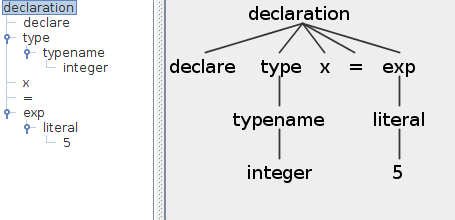
\includegraphics[scale=0.8]{images/pseudo_parse_tree.png}
    \caption{Grafički prikaz stabla parsiranja koje generiše parser kreiran od strane alata ANTLR4 TestRig za kod pisan u pseudo-jeziku.}
    \label{fig:PseudoTreeGui}
\end{figure}


\subsection{Obilazak stabla parsiranja}
\label{subsec:ANTLRParserIntegration}

ANTLR, osim leksera i parsera za datu gramatiku, može da kreira interfejse i bazne klase koji prate obrasce za projektovanje \emph{posetilac} (engl. \emph{visitor}) i osluškivač (engl. \emph{listener}, varijanta obrasca \emph{posmatrač} engl. \emph{observer}) opisane u \ref{sec:DesignPatterns}. Tako kreirani interfejsi i klase imaju metodi za obilazak stabla parsiranja. ANTLR podrazumevano generiše interfejs osluškivača (slika \ref{fig:ANTLRListener}) kao i baznu klasu koja implementira generisani interfejs tako što su sve implementirane metodi prazne. Stoga, ukoliko korisnik želi da definiše operaciju samo u slučaju da se prilikom obilaska stabla parsiranja naiđe na samo jedan tip čvora, nije potrebno implementirati ceo interfejs osluškivača, već je moguće naslediti baznu klasu i predefinisati samo jedan metod. ANTLR može da generiše i posetilac (slika \ref{fig:ANTLRVisitor}), ukoliko se navede odgovarajuća opcija \texttt{-visitor} prilikom pokretanja. Slično, ukoliko nije potrebno generisati osluškivač, može se koristiti opcija \texttt{-no-listener} kako se ne bi generisao osluškivač.

\begin{figure}[h!]
\begin{lstlisting}
public interface IPseudoListener : IParseTreeListener
{
    void EnterUnit([NotNull] PseudoParser.UnitContext context);
    void ExitUnit([NotNull] PseudoParser.UnitContext context);
    void EnterBlock([NotNull] PseudoParser.BlockContext context);
    void ExitBlock([NotNull] PseudoParser.BlockContext context);
    void EnterStatement([NotNull] PseudoParser.StatementContext context);
    void ExitStatement([NotNull] PseudoParser.StatementContext context);
    
    ...
}
\end{lstlisting}
\caption{Delimični prikaz interfejsa osluškivača generisanog od strane ANTLR4 za pseudo-jezik definisan u prethodnom odeljku (C\#).}
\label{fig:ANTLRListener}
\end{figure}

Sa slike \ref{fig:ANTLRListener} se vidi da je moguće definisati metodi koje će se pozivati prilikom ulaska ali i prilikom izlaska iz čvora određenog tipa prilikom obilaska stabla parsiranja. Pritom, važno je kako se stablo obilazi. U slučaju ANTLR, to je pretraga u dubinu (engl. \emph{depth-first search, DFS}) \footnote{DFS je obilazak stabla takav da se obilazak duž grane stabla nastavlja sve dok je moguće ići dublje, a ako to nije moguće vratiti se unazad i obići druge grane.}, stoga će se metod \texttt{Exit} za proizvoljni čvor pozvati tek kad se obiđu sva deca tog čvora - dakle nakon poziva njihovih \texttt{Enter} i \texttt{Exit} metoda. Pošto se DFS obično implementira putem LIFO \footnote{\emph{Last In, First Out} struktura podataka je apstraktna struktura podataka sa operacijama ubacivanja i izbacivanja elemenata, pri čemu je element koji se izbacuje onaj koji je poslednji ubačen. Primer LIFO strukture je držač za CD-ove - ne mogu se ukloniti CD-ovi ispod CD-a na vrhu (poslednji ubačen) a da se ne ukloni isti. U slučaju opisanom iznad, implementacija LIFO strukture se naziva stek \emph{stack}.} strukture, može se reći da se \texttt{Enter} metod poziva onog trenutka kad se čvor ubaci u strukturu, a \texttt{Exit} metod onda kada se čvor ukloni iz strukture.

\begin{figure}[h!]
\begin{lstlisting}
public interface IPseudoVisitor<Result> : IParseTreeVisitor<Result>
{
    Result VisitUnit([NotNull] PseudoParser.UnitContext context);
    Result VisitBlock([NotNull] PseudoParser.BlockContext context);
    Result VisitStatement([NotNull] PseudoParser.StatementContext context);
    Result VisitDeclaration([NotNull] PseudoParser.DeclarationContext context);
    
    ...
}
\end{lstlisting}
\caption{Delimični prikaz interfejsa posetioca generisanog od strane ANTLR4 za pseudo-jezik definisan u prethodnom odeljku (C\#).}
\label{fig:ANTLRVisitor}
\end{figure}

Za razliku od osluškivača, posetilac je prirodnije koristiti ukoliko je potrebno izvršiti neko izračunavanje nad strukturom koja se obilazi. Interfejs posetioca (slika \ref{fig:ANTLRVisitor}) je šablonski, i metodi imaju povratnu vrednost šablonskog tipa za razliku od metoda osluškivača i, u odnosu na osluškivač, nema para metoda za svaki čvor već samo jedan metod. Dodatna razlika, ali i najveća, je ta što se metodi posetioca ne pozivaju automatski. Stoga je na programeru da nastavi obilazak i da odluči u koje čvorove želi da se spusti. Jasno je da i osluškivač i posetilac imaju svoje primene - ukoliko je potrebno obići stablo parsiranja i dovući neke informacije može se iskoristiti osluškivač jer onda ne moramo brinuti o obilasku. S druge strane, ukoliko je potrebno izračunati neku vrednost prirodno je iskoristiti rekurziju i iskoristiti posetilac - rekurzivni pozivi prilikom obilaska nam idu u prilog jer koristimo povratne vrednosti tih metoda da gradimo rezultat od listova ka korenu stabla parsiranja. U nastavku će se koristiti posetilac zbog kontrole obilaska ali i činjenice da se stablo parsiranja obilazi sa ciljem da se izgradi AST, koji je takođe rekurzivna struktura i gradi se inkrementalno kroz rekurziju.

Bilo da se koristi osluškivač ili posetilac, potrebno je nekako proslediti informacije o samom čvoru na koji se naišlo tokom obilaska stabla parsiranja. Te informacije se metodima osluškivača i posetioca prosleđuju putem potklasa apstrakne klase konteksta pravila \texttt{ParserRuleContext} - u primeru iznad \texttt{UnitContext}, \texttt{BlockContext} itd. Svaki kontekst pravila po imenu odgovara pravilima definisanim u gramatici i sadrži informacije bitne za trenutni čvor u stablu parsiranja koji odgovara tipu konteksta. Takođe, u svakom kontekstu su prisutne i metodi čija imena odgovaraju pravilima koja se javljaju u definiciji samog pravila koje odgovara kontekstu. Tako da, za \texttt{BlockContext}, imajući u vidu definiciju sa slike \ref{fig:PseudoDef1}, pošto se u definiciji osim tokena koristi i pravilo \texttt{statement}, u okviru \texttt{BlockContext} klase biće implementiran i metod \texttt{statement()} koji vraća kontekst pravila u ovom slučaju tipa \texttt{StatementContext[]} jer u prvoj alternativi stoji \texttt{statement+} - dakle možemo imati više \texttt{statement} poklapanja. Sa ovim u vidu, moguće je odrediti kako će se obilazak nastaviti (u slučaju posetioca) ili dovući informacije o delovima definicije pravila. Ukoliko pravilo ima više alternativa, metodi koje vraćaju kontekst pravila koje figuriše u alternativi koja nije korišćena za poklapanje pravila će vratiti \texttt{null}. Pošto se \texttt{statement()} pravilo javlja u obe alternative pravila \texttt{block} (i nije opciono), možemo biti sigurni da povratna vrednost \texttt{statement()} metoda nikada neće biti \texttt{null}.

U poglavlju \ref{chp:MyAST} će se koristiti posetilac za obilazak stabla parsiranja i kreiranje AST apstrakcije od istog. Pritom, koristiće se implementacija posetioca u programskom jeziku C\#. Pre toga, potrebno je objasniti pojam \emph{simboličke promenljive} s obzirom da će se ti koncepti koristiti u samoj analizi AST-ova.
